\documentclass[]{report}
\usepackage[parfill]{parskip}
\usepackage{graphicx}

\usepackage{tikz}
\usetikzlibrary{arrows.meta}


% Title Page
\title{Functioneel Ontwerp Codeniacs platform}
\author{Timo Strating - medewerker bij UU-games}
\date{Februari 14, 2017, Groningen}

\renewcommand*\contentsname{Table of Content}
\pagestyle{headings}

\begin{document}
\maketitle

\tableofcontents
\newpage






\chapter{Inleiding}

Het Codeniacs platform heeft als doel om kinderen de mogelijkheid geven om vanaf jongst af aan te leren programmeren / de basis van het programmeren aan te leren.

De Codeniacs projecten bestaat uit meerdere onderdelen waarbij het platform een onderdeel is. Een ander onderdeel is het maandelijkse tijdschrift. Dit tijdschrift moet voor spelletjes, puzzeltjes en meer door kunnen refereren naar het platform. Daarnaast staat er ook een boek in de planning voor het project. Hier geld het zelfde voor.

Het doel van dit platform is dus om een centraal punt te creëren waar naar toe gerefereerd kan worden vanuit andere projecten onder het Codeniacs domein. Dit centrale punt moet een simpel te gebruiken platform zijn waar kinderen zelfstandig kunnen leren programmeren.

De leerstof die wordt aangeboden op het platform zal ondersteund worden door spelletjes mogelijke video’s en een AI die je door het Platform heen begeleid.






\chapter{Belanghebbenden}

\section{Gebruikers}
\begin{itemize}
	\item Kinderen 
	\begin{itemize}
		\item Makkelijk kunnen terug vinden van geleerde onderwerpen.
		\item Zelfstandig kunnen leren van nieuwe dingen.
		\item Het visualiseren van vooruitgang.
			\newline
	\end{itemize} 
	
	\item Beheerders
	\begin{itemize}
		\item Het hebben van een centraal punt waar alle projecten onder het Codeniacs domein zich mee kunnen verbinden.
		\item Het makkelijk kunnen updaten van hun doelgroep.
		\item Het makkelijk kunnen bereiken van hun gebruikers groep.
		\newline
	\end{itemize} 
\end{itemize}


\section{Toekomstige gebruikers}
\begin{itemize}
	
	\item Scholen 
	\begin{itemize}
		\item Een makkelijkere manier van het aanbieden van leerstof die zeer gewild is in de toekomst van onze maatschappij maar nog niet altijd is opgenomen in het huidige school curriculum.
		\newline
	\end{itemize} 
	 
	
	\item Leraren 
	\begin{itemize}
		\item Makkelijker inzicht krijgen in de vooruitgang van de kinderen in hun klaslokalen. 
		\item Het aanbieden van een dynamische leer curve die excellente kinderen makkelijker laat excelleren en een beter inzicht geeft in de kinderen die achter lopen op het gemiddelde.
		\item Een makkelijkere manier van het aanbieden van leerstof die zeer gewild is in de toekomst van onze maatschappij maar nog niet altijd is opgenomen in het huidige school curriculum.
			\newline
	\end{itemize} 
	
	\item Ouders
	\begin{itemize}
		\item Makkelijker inzicht krijgen in de vooruitgang van hun kind. 
		\item Het aanbieden van leerstof die zeer gewild is in de toekomst van onze maatschappij maar nog niet altijd is opgenomen in het huidige school curriculum.
			\newline
	\end{itemize} 

	\item Coaches
	\begin{itemize}
		\item Makkelijker inzicht krijgen in de vooruitgang van het kind. 
		\item Beter advies kunnen geven door een beter inzicht in de analyse van het kind zijn leer curve. 
			\newline
	\end{itemize} 
\end{itemize}







\chapter{Behoeftes}

\begin{itemize}
	\item Kinderen - Het makkelijker en leuker leren van programmeren .	
	\item Ouders - Het aanbieden van lesstof op een spelende wijs waarin de kinderen zichzelf zullen excelleren. 
	\item Scholen - Een makkelijkere manier van het aanbieden van leerstof die zeer gewild is in de toekomst van onze maatschappij maar nog niet altijd is opgenomen in het huidige school curriculum
	\item Leraren / Couches - Het hebben van stabiel en toekomst uitbreidend platform dat de leercurve van de leerlingen excelleert. 
	\item Beheerders - Het hebben van een centraal systeem dat meerdere projecten uit het Codeniacs domein verbind / versterkt.
	\item Andere Codeniacs projecten - Het hebben van een centraal platform waar naar gerefereerd kan worden om meer informatie / de andere content te vergaren. Deze verbindingen worden zowel als simpele referenties gedaan als leuke QR codes en puzzeltjes.
	
\end{itemize}






\chapter{Functionaliteiten}

\textit{In het archief staat een spelletje hier kan een kind op klikken zodat hij het kan gaan spelen.}

Beheerders moeten kunnen inloggen. \\
Beheerders moeten alle content kunnen zien. \\
Beheerders moeten nieuwe game kunnen aanmaken. \\
\\

\textit{Op de dashboard reageert de AI met "hee misschien is deze video ook leuk".}

Beheerders moeten kunnen inloggen. \\
Beheerders moeten alle content kunnen zien. \\
Beheerders moeten nieuwe video kunnen aanmaken. \\
Gebruiker moet kunnen inloggen. \\ 
Het AI systeem moet de situatie analyseren. \\
Het AI systeem moet automatisch advies kunnen geven aan de gebruiker op basis van de analyse. \\
\\


\textit{In de dashboard ziet de gebruiker statistieken over zijn vooruitgang.}

Beheerders moeten kunnen inloggen. \\
Beheerders moeten alle content kunnen zien. \\
Beheerders moeten nieuwe quizes kunnen aanmaken. \\
Gebruiker moet kunnen inloggen. \\ 
Het systeem moet kunnen bijhouden welke onderwerpen er zijn. \\ 
Het systeem moet kunnen bijhouden welke onderwerpen voltooid zijn door de gebruiker. \\ 
Het systeem moet statistieken genereren op basis van de voltooide onderwerpen. \\





\chapter{Navigatie}
%%%%%%%%%%%%%%%%%%%%%%%%%%%%%%%%%%%%%%%%%%%%%%%%%%%%%%%%%%%%%%%%%
%   http://www.texample.net/tikz/examples/android/              %
%   http://www.texample.net/tikz/examples/simple-flow-chart/    %
%%%%%%%%%%%%%%%%%%%%%%%%%%%%%%%%%%%%%%%%%%%%%%%%%%%%%%%%%%%%%%%%%
\tikzset{ >={Latex[width=2mm,length=2mm]},
	% Specifications for style of nodes:
	base/.style = {rectangle, rounded corners, draw=black, minimum width=2.5cm, minimum height=0.75cm, text centered, font=\ttfamily},
	blue/.style = {base, fill=blue!30},
	yellow/.style = {base, fill=orange!15},
	green/.style = {base, fill=green!15},
}
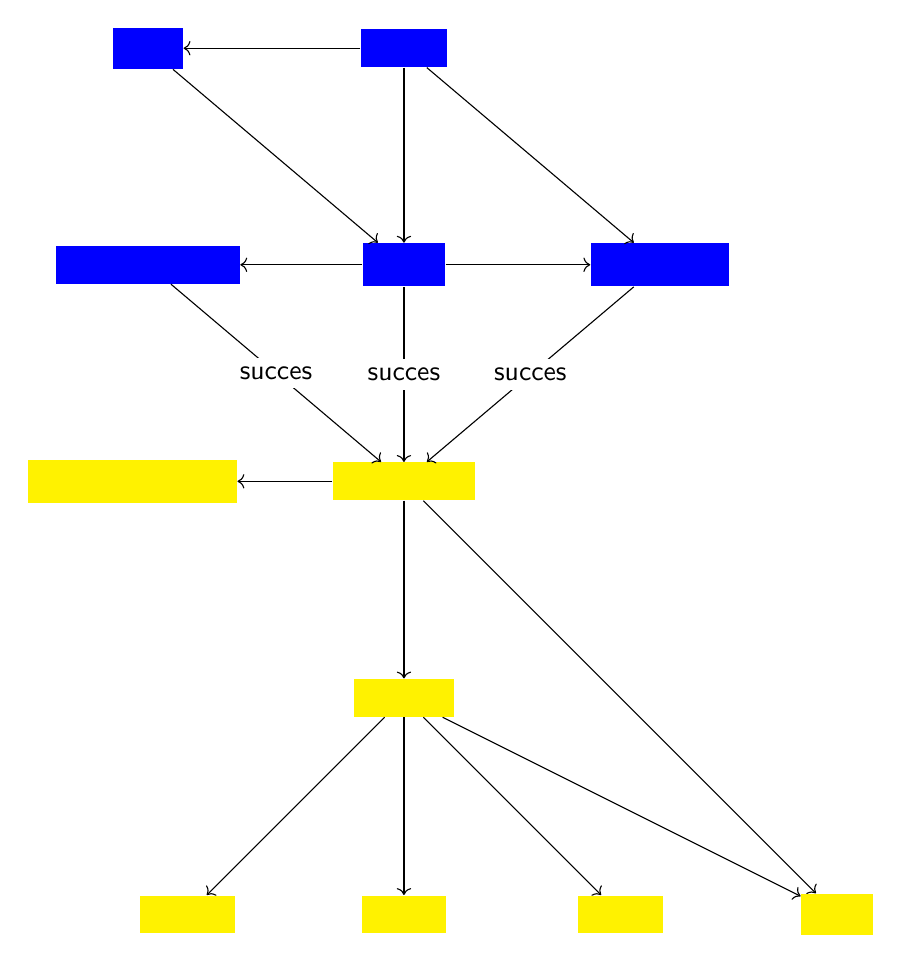
\begin{tikzpicture}[ node distance=2.75cm, every node/.style={fill=white, font=\sffamily}, align=center]
% Specification of nodes (position, etc.)

\node (home)              	[blue]              						{Home};
\node (faq)              	[blue, left of=home, xshift=-0.5cm]        	{FAQ};

\node (login)     		  	[blue, below of=home]      					{Login};
\node (register)      	 	[blue, right of=login, xshift=0.5cm]   		{Registeren};
\node (lostPassword)     	[blue, left of=login, xshift=-0.5cm]   		{Lost Password};

\node (dashboard)     		[yellow, below of=login]      				{Dashboard};
\node (userpage)      	 	[yellow, left of=dashboard, xshift=-0.7cm]   	{gebruikerspagina};

\node (archive)      	 	[yellow, below of=dashboard]   				{Archief};

\node (content-video)  		[yellow, below of=archive]   				{Video};
\node (content-artikel)  	[yellow, left of=content-video]   			{Artikel};
\node (content-game)     	[yellow, right of=content-video]   			{Game};
\node (content-quiz)     	[yellow, right of=content-game]   			{Quiz};

\draw[->]             (home) -- (login);
\draw[->]             (home) -- (register);
\draw[->]             (home) -- (faq);
\draw[->]             (faq) -- (login);
\draw[->]             (login) -- (register);
\draw[->]             (login) -- (lostPassword);

\draw[->]             (lostPassword) -- node {succes} (dashboard);
\draw[->]             (login) -- node {succes}(dashboard);
\draw[->]             (register) -- node {succes}(dashboard);

\draw[->]             (dashboard) -- (userpage);
\draw[->]             (dashboard) -- (archive);

\draw[->]             (archive) -- (content-video);
\draw[->]             (archive) -- (content-artikel);
\draw[->]             (archive) -- (content-game);
\draw[->]             (archive) -- (content-quiz);

\draw[->]             (dashboard) -- (content-quiz);

\end{tikzpicture}







\chapter{Paginalijst}

\section{Publiekelijke Pagina's}

\begin{tabular}{ l l p{6cm} }
	\textbf{Naam} & \textbf{Formulier} & \textbf{Functie} \\ \hline
	Home 				& Nee		& Dit is de eerste pagina die mensen zien als ze naar de website navigere.n \\ 
	Login 				& Ja		& Hier kan een kind inloggen. \\
	Register 			& Ja		& Hier kan een kind zich inschrijven voor het platform \\
	Lost Password		& Ja		& Deze pagina kan worden gebruikt om het wachtwoord opnieuw aan te vragen of via Sociaal media in te loggen. \\
	FAQ 				& Ja 		& Hier kunnen de meest gestelde vragen worden bekeken, en desnoods als het nodig is een nieuwe vraag gesteld worden. \\
\end{tabular}


\section{Backend}
\begin{tabular}{ p{4cm} l p{6cm} }
	\textbf{Naam} & \textbf{Formulier} & \textbf{Functie} \\ \hline
	Backend login	& -		& Hier kan er in worden ingelogd door de beheerders van het platform. \\
	Backend users	& - 	& Hier kunnen alle gebruikers bekeken worden. \\
	Backend content & - 	& Hier kan er nieuwe content aan het Platform worden toegevoegd. \\
\end{tabular}


\section{Pagina's Beschikbaar na login}
\begin{tabular}{ p{4cm} l p{6cm} }
	\textbf{Naam} & \textbf{Formulier} & \textbf{Functie} \\ \hline
	Dashboard progress 	& Nee		& Hier kan de gebruiker zien hoe ver hij is en wat zijn volgende stappen kunnen zijn. Dit is de standaard dashboard. \\
	Dashboard gebruiker	& Ja		& Hier kan de gebruiker gegevens van zijn account inzien en veranderen. \\
	Archief 			& Ja		& Dit is het overzicht van alle categorieën en alle opdrachten / puzzeltjes die op het platform te vinden zijn. \\ 
	Archief zoekresultaten	& Ja 	& Dit is een speciale verzie van het Archief dat de gebruiker toont waar hij naar gezocht heeft. Deze pagina is gelijk aan het normale Archief en is daarom niet opgenomen als aparte pagina ook al ziet de gebruiker dit als aparte pagina.  \\
	Content artikel 	& Nee		& Hier kan de content in de vorm van een artikel bekeken worden.  \\
	Content video 		& Nee 		& Hier kan de content in de vorm van een video bekeken worden. \\
	Content game 		& Nee 		& Hier kan een spelletje worden gespeeld om spelende wijs de gebruiker lesstof mee te geven. \\
	Content quiz 		& Ja 		& Hier kan een quiz worden gedaan om te testen wat je kennis is. \\
\end{tabular}







\chapter{Paginaontwerp}

\section{Pagina's Beschikbaar na login}
\begin{tabular}{ l l p{6cm} }
	\textbf{Pagina} & \textbf{Figuur} & \textbf{Uitleg}\\ \hline
	Home 					& \ref{fig:wireframe-home}	\\
	FAQ 					& \ref{fig:wireframe-faq}	\\
	Login 					& \ref{fig:wireframe-login}	\\
	Register 				& \ref{fig:wireframe-register}	\\
	Lost Password			& \ref{fig:wireframe-lostPassword} \\
	Dashboard progress 		& \ref{fig:wireframe-dashboard-progress}	\\
	Dashboard gebruiker		& \ref{fig:wireframe-dashboard-user}	\\
	Archief 				& \ref{fig:wireframe-archive}	\\
	Archief zoekresultaten	& \ref{fig:wireframe-archive}	& Het archief voor de zoekresultaten is gelijk aan het archief alleen dan gevuld met items waar naar gezocht wordt.\\
	Content artikel 		& \ref{fig:wireframe-content-artikel}	\\
	Content video 			& \ref{fig:wireframe-content-video} 	\\
	Content game 			& \ref{fig:wireframe-content-artikel} / \ref{fig:wireframe-content-video}	& \\
	Content quiz 			& \ref{fig:wireframe-content-artikel} / \ref{fig:wireframe-content-video}  & De quiz game krijgt een pagina vergelijkbaar met de content pagina's. \\
\end{tabular}

\section{Ontwerpen}

\begin{figure}
	\centering
	\includegraphics[scale=0.4]{wireframe-home}
	\caption{wireframe-home}
	\label{fig:wireframe-home}
\end{figure}

\begin{figure}
	\centering
	\includegraphics[scale=0.4]{wireframe-faq}
	\caption{wireframe-faq}
	\label{fig:wireframe-faq}
\end{figure}

\begin{figure}
	\centering
	\includegraphics[scale=0.4]{wireframe-login}
	\caption{wireframe-login}
	\label{fig:wireframe-login}
\end{figure}


\begin{figure}
	\centering
	\includegraphics[scale=0.4]{wireframe-register}
	\caption{wireframe-register}
	\label{fig:wireframe-register}
\end{figure}

\begin{figure}
	\centering
	\includegraphics[scale=0.4]{wireframe-lostPassword}
	\caption{wireframe-lostPassword}
	\label{fig:wireframe-lostPassword}
\end{figure}


\begin{figure}
	\centering
	\includegraphics[scale=0.4]{wireframe-dashboard-progress}
	\caption{wireframe-dashboard-progress}
	\label{fig:wireframe-dashboard-progress}
\end{figure}

\begin{figure}
	\centering
	\includegraphics[scale=0.4]{wireframe-dashboard-user}
	\caption{wireframe-dashboard-user}
	\label{fig:wireframe-dashboard-user}
\end{figure}

\begin{figure}
	\centering
	\includegraphics[scale=0.4]{wireframe-archive}
	\caption{wireframe-archive}
	\label{fig:wireframe-archive}
\end{figure}

\begin{figure}
	\centering
	\includegraphics[scale=0.4]{wireframe-content-artikel}
	\caption{wireframe-content-artikel}
	\label{fig:wireframe-content-artikel}
\end{figure}

\begin{figure}
	\centering
	\includegraphics[scale=0.4]{wireframe-content-video}
	\caption{wireframe-content-video}
	\label{fig:wireframe-content-video}
\end{figure}









\chapter{formulierontwerp}

De formulier ontwerpen zijn opgenomen in de ontwerpen van de pagina's.
de volgende pagina's bevatten een formulier: 

\begin{tabular}{ l l p{6cm} }
	\textbf{Naam} & \textbf{Formulier} & \textbf{Functie} \\ \hline
	Login Kinderen 		& Ja		& Hier kan een kind inloggen. \\
	FAQ 				& Ja 		& Hier kunnen kunnen vragen gesteld worden. \\
	Dashboard gebruiker	& Ja		& Hier kan de gebruiker gegevens van zijn account inzien en veranderen. \\
	Archief 			& Ja		& Hier is een zoekbalk die de gebruiker kan gebruiken om specifieke content makkelijker te vinden. \\
	Content game 		& - 		& De content van het Platform zal worden aangeleverd en is daarom niet een onderdeel van de opdracht. \\
	Content quiz 		& - 		& De Quizes zijn een onderdeel van de content, zie "Content game". \\
\end{tabular}






\chapter{Grafischontwerp}

\section{Inleiding}
Het grafisch ontwerp zal worden aangeleverd door een extern team en is geen onderdeel van de opdracht. Indien het aangeleverd is zal het Grafischontwerp worden opgenomen in dit document en zal het mee worden genomen in de realisatie van het project.

\section{Richtlijnen}
Omdat het grafisch ontwerp door een extern team zal worden ontwikkeld zullen niet alle richtlijnen worden opgenomen worden in de Definition of Done. Om deze reden volgt hier een overzichtje met richtlijnen waar de optelveren documenten aan dienen voldoen om meegenomen te kunnen worden in de realisatie van het project.

\vspace{5mm} %5mm vertical space

\begin{itemize}
	\item Alle gebruikte afbeeldingen in het grafischontwerp dienen onderbouwd te zijn met een geldige licentie.
	\item Alle bestanden dienen als bronbestanden en als web geoptimaliseerde versie te worden opgeleverd.
	\begin{itemize}
		\item Bronbestanden - onder bronbestanden wordt verstaan: het bestand dat gebruikt is om het uiteindelijke bestand te kunnen exporteren. Dit bestandstype dient geopend te kunnen worden zonder te veel moeite / externe Programma's Het is daarom belangrijk dat er een gangbaar bestandstype word gekozen voor de bronbestanden.
		\item Web geoptimaliseerde versie - het bronbestand dient ge\"{e}xporteerd te worden als gecomprimeerd png bestand. daarnaast dienen alle extern gebruikte afbeeldingen in het brondbestand correct uitgeknipt mee ge\"{e}xporteerd te worden als losse gecomprimeerd png bestanden. Deze losse bestanden dienen ieder aan richtlijn 1 te voldoen.
		\newline
	\end{itemize} 
	\item Alle designs dienen te voldoen aan het 12 cellig grid systeem van Twitter bootstrap.
	\item Alle designs dienen te voldoen aan de Google material design filosofie.
	\item Alle designs dienen als 3 versies opgeleverd te worden: mobiel, tablet en latop/pc.
	\newline
\end{itemize} 



\end{document}      
